\documentclass[a4paper,12pt]{report}
\usepackage{graphicx}
\graphicspath{{picaa/}}
\usepackage{listings}
\usepackage{amsmath}
\usepackage[T2A]{fontenc}
\usepackage[utf8]{inputenc}
\usepackage[english,russian]{babel}
\usepackage{pgfplots} 
\usepackage{indentfirst}
\parindent=1cm

\usepackage{geometry}
\geometry{left=2cm}
\geometry{right=1.5cm}
\geometry{top=1cm}
\geometry{bottom=2cm}
\lstset{language = Python,
keywordstyle = \color{orange},
stringstyle = \color{green},
commentstyle = \color{red},
columns = fullflexible,
captionpos = t
}

\begin{document}

    \begin{titlepage}

        \begin{center}
            \large
            \textbf{Государственное образовательное учреждение высшего профессионального образования\\
            “Московский государственный технический университет имени Н.Э.Баумана”\\}
            
\includegraphics{bmstu-logo.png}
			\vspace{1cm}
            
            \textsc{Дисциплина: Анализ алгоритмов}
            \vspace{0.5cm}
                
            \textsc{Рубежный контроль №1}
            \vspace{1cm}
            
            {\LARGE \textbf{Нахождение клик наиболее эффективным способом}}
            \vspace{3cm}
                    
            \begin{flushright}
            	Студент группы ИУ7-55Б,\\   
            	Руднев К. К.,\\
            	\vspace{0.5cm}
            	Преподаватель,\\
            	Волкова Л. Л.,\\
            	Строганов Ю. В.
            	
            \end{flushright}
            \vfill
            
            2019 г.
            
        \end{center}

    \end{titlepage}

	\setcounter{page}{2}
    \newpage

    \begin{center}
        \textbf{1 Аналитическая часть}
    \end{center}
        \label{sec:analitic_part}

        	В рамках раздела будет дано аналитическое описание алгоритма Брона-Кербоша для нахождения всех клик в графе.

	\begin{center}
        \textbf{1.1 Описание алгоритмов}
    \end{center}
        
	       Алгоритм Брона-Кербоша - метод ветвей и границ для поиска всех клик (а также максимальных по включению независимых множеств вершин) неориентированного графа. Разработан голландскими математиками Броном и Кербошем в 1973 году и до сих пор является одним из самых эффективных алгоритмов поиска клик.
	       
	       Алгоритм использует тот факт, что всякая клика в графе является его максимальным по включению полным подграфом. Начиная с одиночной вершины (образующей полный подграф), алгоритм на каждом шаге пытается увеличить уже построенный полный подграф, добавляя в него вершины из множества кандидатов. Высокая скорость обеспечивается отсечением при переборе вариантов, которые заведомо не приведут к построению клики, для чего используется дополнительное множество, в которое помещаются вершины, которые уже были использованы для увеличения полного подграфа.
	       \vspace{0.5cm}
	       
	       Алгоритм можно представить в виде рекурсивной процедуры:\\
	       ПРОЦЕДУРА extend (candidates, not):\\
	       ПОКА candidates НЕ пусто И not НЕ содержит вершины, СОЕДИНЕННОЙ СО ВСЕМИ вершинами из candidates, 
	       ВЫПОЛНЯТЬ:\\
	       1 Выбрать вершину v из candidates и добавить её в compsub\\
	       2 Формировать new\_candidates и new\_not, удаляя из candidates и not вершины, не СОЕДИНЕННЫЕ с v\\
	       3 ЕСЛИ new\_candidates и new\_not пусты\\
	       4 ТО compsub – клика\\
	       5 ИНАЧЕ рекурсивно вызвать extend (new\_candidates, new\_not)\\
	       6 Удалить v из compsub и candidates и поместить в not\\

    \newpage

    \begin{center}
        \textbf{2 Конструкторская часть}
    \end{center}
        \label{sec:construct_part}

			В дальнейшем на рисунке \ref{ris:bron_k} будет представлена схема расматриваемого алгоритма.

	\begin{center}
        \textbf{2.1 Разработка алгоритмов}
    \end{center}

		\begin{figure}[h!]
			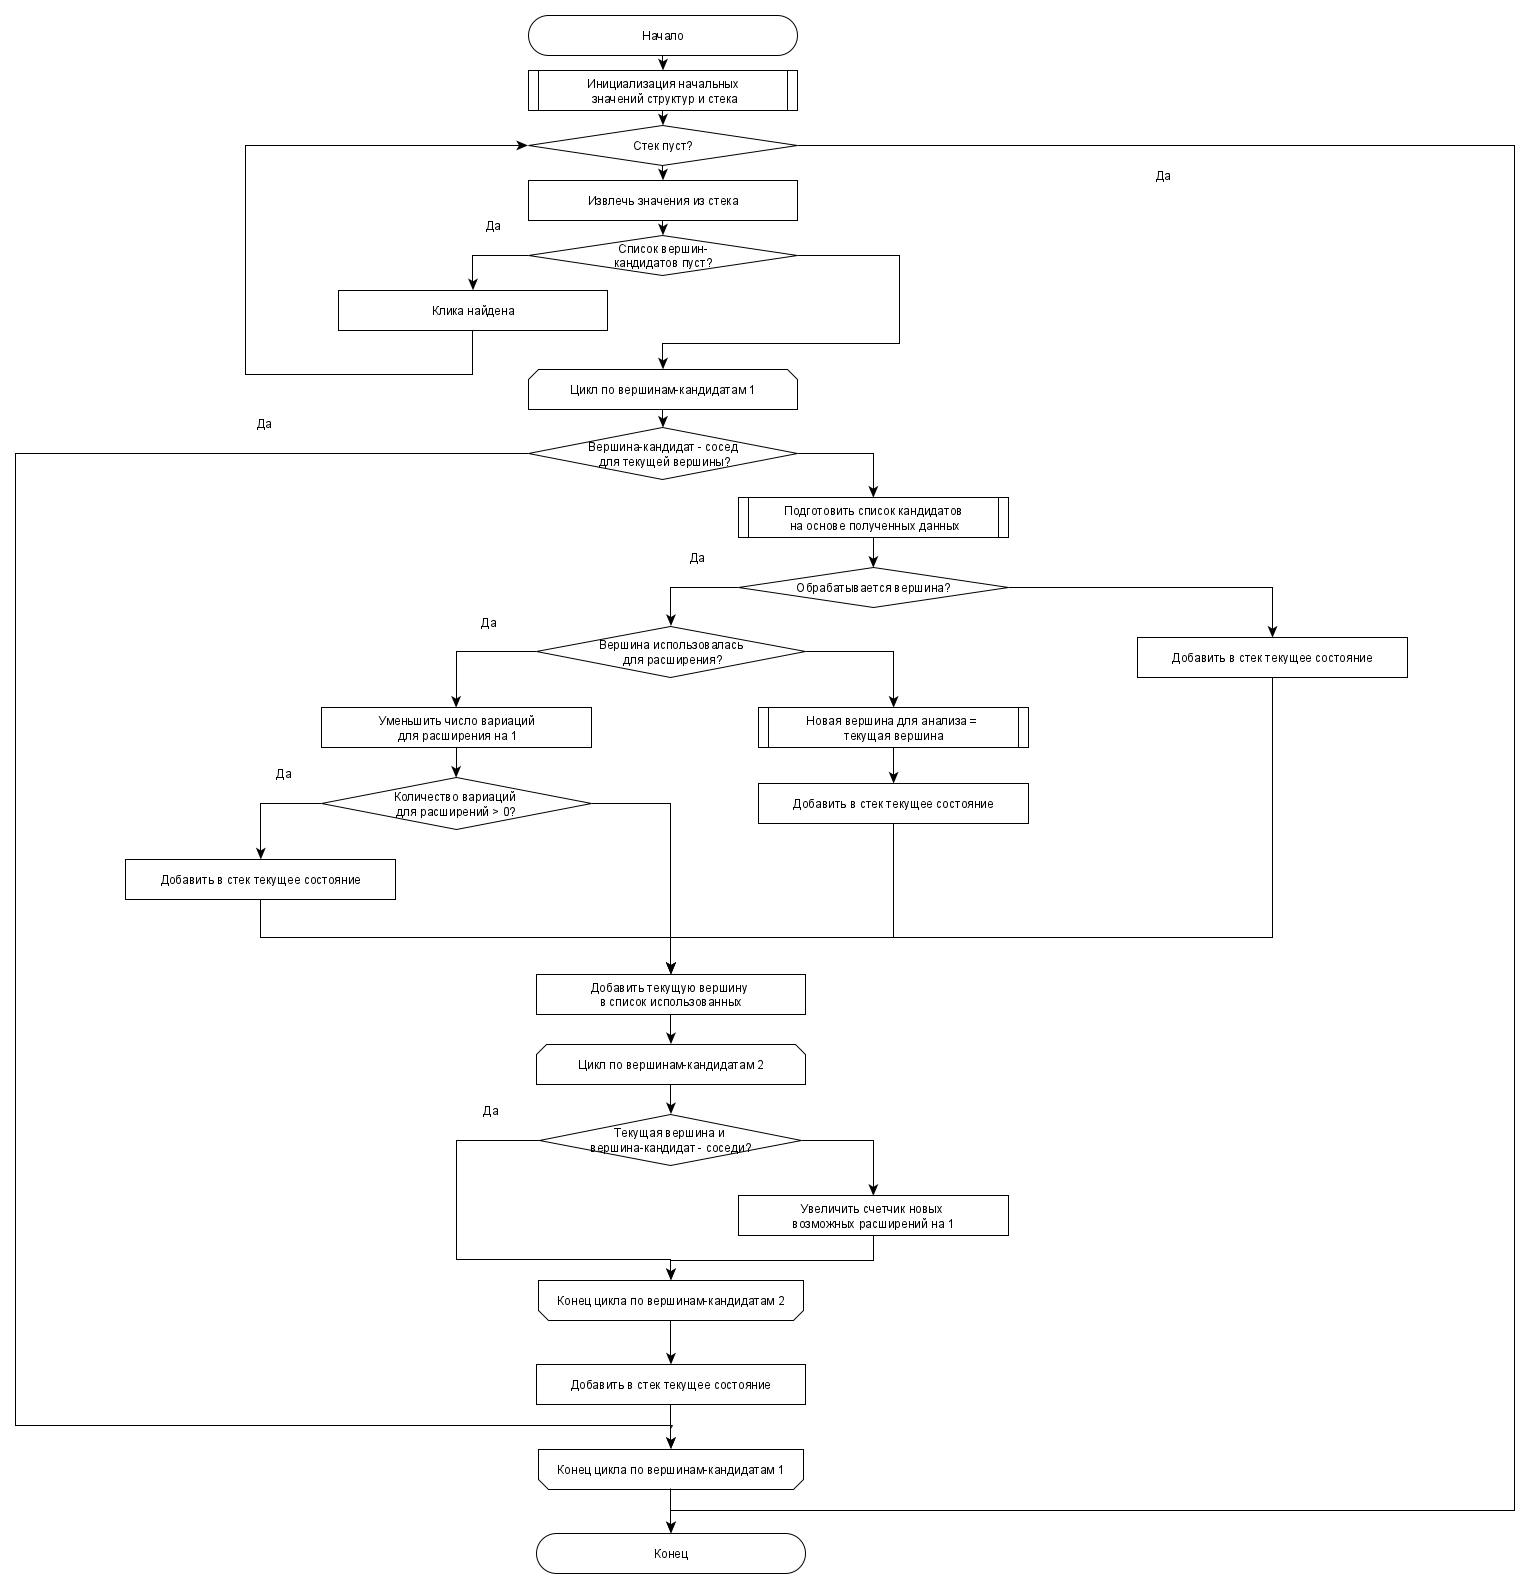
\includegraphics[width=1\linewidth]{bron_kerbosh.png}
			\caption{Алгоритм Брона-Кербоша}
			\label{ris:bron_k}
		\end{figure}

    \newpage

    \begin{center}
        \textbf{3 Технологическая часть}
    \end{center}
        \label{sec:tecnologic_part}

			В рамках раздела будут описаны инструментарии разработки, выбор среды, требования к ПО. 
			Также будут предоставлены листинги конкретных реализаций алгоритмов.

	\begin{center}	
        \textbf{3.1. Средства реализации}
    \end{center}

        	Для реализации алгоритмов использовался язык программирования Python 3.8.0 и среда разработки PyCharm Community Edition 2019.3.1 by JetBrains. 
        	У меня есть определенный опыт работы с данным языком, которого будет достаточно для реализации текущей лабораторной работы, а среда разработки имеет бесплатную комьюнити версию и удобный интерфейс, упрощающий разработку приложения/скрипта.\\

	\begin{center}
		\textbf{3.2. Требования к программному обеспечению}
	\end{center}

			На вход программа должна получать граф, на выход отображать все существующие в этом графе клике.
	
	\begin{center}
		\textbf{3.3. Листинг кода}
	\end{center}

	        \begin{lstlisting}[frame = single, breaklines, caption = Листинг метода поиска всех существующих клик в графе]
	def find_all_cliques(self):
	    Cliques = []
	    Stack = []
	    nd = None
	    disc_num = len(self.Nodes)
	    search_node = (set(), set(self.Nodes), set(), nd, disc_num)
	    Stack.append(search_node)
	    while len(Stack) != 0:
	    	(c_compsub, c_candidates, c_not, c_nd, c_disc_num) = Stack.pop()
	        if not len(c_candidates) and c_compsub not in Cliques:
	        	Cliques.append(c_compsub)
	        	continue
	        for u in list(c_candidates):
	        	if (c_nd is None) or (not self.are_adjacent(u, c_nd)):
	        		c_candidates.remove(u)
	        		Nu = self.get_node_neighbors(u)
	        		new_compsub = set(c_compsub)
	        		new_compsub.add(u)
	        		new_candidates = set(c_candidates.intersection(Nu))
	        		new_not = set(c_not.intersection(Nu))
	        		if c_nd is not None:
	        			if c_nd in new_not:
	        				new_disc_num = c_disc_num - 1
	        				if new_disc_num > 0:
	        					new_search_node = (new_compsub, new_candidates, new_not, c_nd, new_disc_num)
	        					Stack.append(new_search_node)
	        				else:
	        					new_disc_num = len(self.Nodes)
	        					new_nd = c_nd
	        		for cand_nd in new_not:
	        			cand_disc_num = len(new_candidates) - len(new_candidates.intersection(self.get_node_neighbors(cand_nd)))
	        			if cand_disc_num < new_disc_num:
	        				new_disc_num = cand_disc_num
	        				new_nd = cand_nd
	        		new_search_node = (new_compsub, new_candidates, new_not, new_nd, new_disc_num)
	        		Stack.append(new_search_node)
	        else:
	        	new_search_node = (new_compsub, new_candidates, new_not, c_nd, c_disc_num)
	        	Stack.append(new_search_node)
	        c_not.add(u)
	        new_disc_num = 0
	        for x in c_candidates:
	        	if not self.are_adjacent(x, u):
	        		new_disc_num += 1
	        if (new_disc_num < c_disc_num) and (new_disc_num > 0):
	        	new1_search_node = (c_compsub, c_candidates, c_not, u, new_disc_num)
	        	Stack.append(new1_search_node)
	        else:
	        	new1_search_node = (c_compsub, c_candidates, c_not, c_nd, c_disc_num)
	        	Stack.append(new1_search_node)
	    while set() in Cliques:
	    	Cliques.pop(Cliques.index(set()))
	    return Cliques
	        \end{lstlisting} 	

    \newpage

    \begin{center}
        \textbf{Заключение}
    \end{center}
        \label{sec:conclusion_part}
        
   		Выполнен рубежный контроль по поиску клик эффективным способом. 
   		Изучен и реализован алгоритм Брона-Кербоша.

\end{document}
